% Partial reconstruction: genuine architectural drawing retained; analytic section rebuilt in TikZ.
\begin{minipage}[c]{5.1cm}\centering
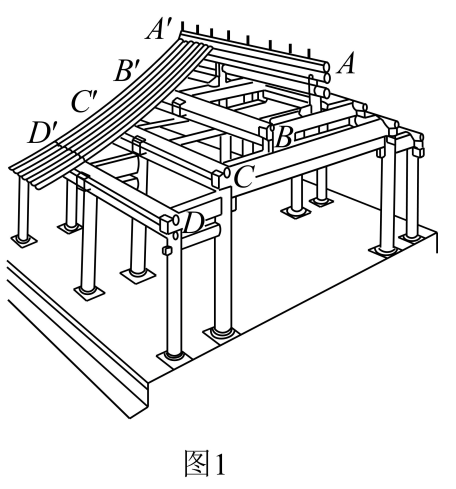
\includegraphics[width=5.1cm,trim=0 70bp 0 0,clip]{img/2022/new_gaokao_paper_2/q3_fig1_architecture.png}\\\bitmapinsertcaption[1]
\end{minipage}\hspace{.4cm}
\begin{minipage}[c]{11.2cm}\centering
% Equal horizontal steps. D,C,B,A are on the roof; D1,C1,B1,A1 are feet of successive rises.
% Coordinates satisfy the source's arithmetic sequence of rises and OA slope .725, with no answer annotation.
\begin{tikzpicture}[x=1.02cm,y=1.02cm,line width=.6pt,font=\normalsize,>=Stealth]
\draw[->] (0,0)--(8.65,0) node[right,inner sep=2pt] {$x$};
\draw[->] (0,0)--(0,3.9) node[above,inner sep=2pt] {$y$};
\draw (0,0)--(1,.5)--(2,1.2)--(3,2)--(4,2.9)--(5,2)--(6,1.2)--(7,.5)--(8,0);
\draw (1,0)--(1,.5)--(7,.5)--(7,0);
\draw (2,.5)--(2,1.2)--(6,1.2)--(6,.5);
\draw (3,1.2)--(3,2)--(5,2)--(5,1.2);
\draw (4,2)--(4,2.9);
\node[anchor=north east,inner sep=2pt] at (0,0) {$O$};
\node[anchor=south east,inner sep=2pt] at (1,.5) {$D$};
\node[anchor=south east,inner sep=2pt] at (2,1.2) {$C$};
\node[anchor=south east,inner sep=2pt] at (3,2) {$B$};
\node[anchor=south,inner sep=2pt] at (4,2.9) {$A$};
\node[anchor=north,inner sep=2pt] at (1,0) {$D_1$};
\node[anchor=north,inner sep=2pt] at (2,.5) {$C_1$};
\node[anchor=north,inner sep=2pt] at (3,1.2) {$B_1$};
\node[anchor=north,inner sep=2pt] at (4,2) {$A_1$};
\end{tikzpicture}
\\\bitmapinsertcaption[2]
\end{minipage}
